\documentclass{book}

\usepackage{fontspec} % used to import Calibri
\usepackage{anyfontsize} % used to adjust font size

% needed for inch and other length measurements
% to be recognized
\usepackage{calc}

% for colors and text effects as is hopefully obvious
\usepackage[dvipsnames]{xcolor}
\usepackage{soul}

% control over margins
\usepackage[margin=1in]{geometry}
\usepackage[strict]{changepage}

\usepackage{mathtools}
\usepackage{amsfonts}
\usepackage{bm}

\usepackage[scr=rsfso, scrscaled=.96]{mathalpha}

\usepackage{amssymb} % originally imported to get the proof square
\usepackage{xfrac}
\usepackage[overcommands]{overarrows} % Get my preferred vector arrows...
\usepackage{relsize}

% Just am using this to get a dashed line in a table...
% Also you apparently want this to be inactive if you aren't
% using it because it slows compilation.
\usepackage{arydshln} \ADLinactivate 
\newenvironment{allowTableDashes}{\ADLactivate}{\ADLinactivate}

\usepackage{graphicx}
\graphicspath{{./158_Images/}}

\usepackage{tikz}
   \usetikzlibrary{arrows.meta}
   \usetikzlibrary{graphs, graphs.standard}

\usepackage{quiver} %commutative diagrams


\newfontfamily{\calibri}{Calibri}
\setlength{\parindent}{0pt}
\definecolor{RawerSienna}{HTML}{945D27}

% ~~~~~~~~~~~~~~~~~~~~~~~~~~~~~~~~~~~~~~~~~~~~~~~~~~
%Arrow Commands:

% Thank you Bernard, gernot, and Sigur who I copied this from:
% https://tex.stackexchange.com/questions/364096/command-for-longhookrightarrow
\newcommand{\hooklongrightarrow}{\lhook\joinrel\longrightarrow}
\newcommand{\hooklongleftarrow}{\longleftarrow\joinrel\rhook}
\newcommand{\hookxlongrightarrow}[2][]{\lhook\joinrel\xrightarrow[#1]{#2}}
\newcommand{\hookxlongleftarrow}[2][]{\xleftarrow[#1]{#2}\joinrel\rhook}

% Thank you egreg who I copied from:
% https://tex.stackexchange.com/questions/260554/two-headed-version-of-xrightarrow
\newcommand{\longrightarrowdbl}{\longrightarrow\mathrel{\mkern-14mu}\rightarrow}
\newcommand{\longleftarrowdbl}{\leftarrow\mathrel{\mkern-14mu}\longleftarrow}

\newcommand{\xrightarrowdbl}[2][]{%
  \xrightarrow[#1]{#2}\mathrel{\mkern-14mu}\rightarrow
}
\newcommand{\xleftarrowdbl}[2][]{%
  \leftarrow\mathrel{\mkern-14mu}\xleftarrow[#1]{#2}
}

\newcommand{\MRoman}[1]{%
   \textrm{\MakeUppercase{\romannumeral #1}}%
}

% ~~~~~~~~~~~~~~~~~~~~~~~~~~~~~~~~~~~~~~~~~~~~~~~~~~

\newcommand{\learnToSpot}[1]{{\color{Red}#1}}

\newcommand{\hOne}{%
   \color{Black}%
   \fontsize{14}{16}\selectfont%
}
\newcommand{\hTwo}{%
\color{MidnightBlue}%
   \fontsize{13}{15}\selectfont%
}
\newcommand{\hThree}{%
   \color{PineGreen!85!Orange}
   \fontsize{12}{14}\selectfont%
}
\newcommand{\hFour}{%
   \color{Cyan}
   \fontsize{12}{14}\selectfont%
}
\newcommand{\myComment}{%
   \color{RawerSienna}%
   \fontsize{12}{14}\selectfont%
}
\newcommand{\teachComment}{
   \color{Orange}%
   \fontsize{12}{14}\selectfont%
}
\newcommand{\exOne}{%
   \color{Purple}%
   \fontsize{13}{15}\selectfont%
}
\newcommand{\exTwo}{%
   \color{Purple}%
   \fontsize{13}{15}\selectfont%
}
\newcommand{\exP}{%
   \color{Purple}%
   \fontsize{12}{14}\selectfont%
}
\newcommand{\exTwoP}{%
   \color{RedViolet}%
   \fontsize{13}{15}\selectfont%
}
\newcommand{\exPP}{%
   \color{RedViolet}%
   \fontsize{12}{14}\selectfont%
}
% ~~~~~~~~~~~~~~~~~~~~~~~~~~~~~~~~~~~~~~~~~~~~~~~~

\newcommand{\cyPen}[1]{{\vphantom{.}\color{Cerulean}#1}}
\newcommand{\redPen}[1]{{\vphantom{.}\color{Red}#1}}

\newenvironment{myIndent}{%
   \begin{adjustwidth}{2.5em}{0em}%
}{%
   \end{adjustwidth}%
}

\newenvironment{myDindent}{%
   \begin{adjustwidth}{5em}{0em}%
}{%
   \end{adjustwidth}%
}

\newenvironment{myTindent}{%
   \begin{adjustwidth}{7.5em}{0em}%
}{%
   \end{adjustwidth}%
}

\newenvironment{myConstrict}{%
   \begin{adjustwidth}{2.5em}{2.5em}%
}{%
   \end{adjustwidth}%
}

\newcommand{\udefine}[1]{{%
   \setulcolor{Red}%
   \setul{0.14em}{0.07em}%
   \ul{#1}%
}}

\newcommand{\blab}[1]{\textbf{#1}}

\newcommand{\uuline}[2][.]{%
{\vphantom{a}\color{#1}%
\rlap{\rule[-0.18em]{\widthof{#2}}{0.06em}}%
\rlap{\rule[-0.32em]{\widthof{#2}}{0.06em}}}%
#2}

\newcommand{\pprime}{{\prime\prime}}
\newcommand{\suchthat}{ \hspace{0.3em}s.t.\hspace{0.3em}}
\newcommand{\rea}[1]{\mathrm{Re}(#1)}
\newcommand{\ima}[1]{\mathrm{Im}(#1)}
\newcommand{\comp}{\mathsf{C}}
\newcommand{\card}{\mathrm{card}}
\newcommand{\diam}{\mathrm{diam}}
\newcommand{\myHS}{ \hspace{0.5em}}

\newcommand{\myId}{\mathrm{Id}}
\newcommand{\myIm}{\mathrm{im}}
\newcommand{\myObj}{\mathrm{Obj}}
\newcommand{\myHom}{\mathrm{Hom}}
\newcommand{\myEnd}{\mathrm{End}}
\newcommand{\myAut}{\mathrm{Aut}}

\newcommand{\mcateg}[1]{{\bm{\mathsf{#1}}}}

\newcommand{\mdeg}{\mathrm{mdeg}\phantom{.}}

% Thank you Gonzalo Medina and Moriambar who wrote this on stack exchange:
%https://tex.stackexchange.com/questions/74125/how-do-i-put-text-over-symbols%
\newcommand{\myequiv}[1]{\stackrel{\mathclap{\mbox{\footnotesize{$#1$}}}}{\equiv}}

% Thank you chs who wrote this on stack exchange:
%https://tex.stackexchange.com/questions/89821/how-to-draw-a-solid-colored-circle%
\newcommand{\filledcirc}[1][.]{\ensuremath{\hspace{0.05em}{\color{#1}\bullet}\mathllap{\circ}\hspace{0.05em}}}

%Thank you blerbl who wrote this on stack exchange:
%https://tex.stackexchange.com/questions/25348/latex-symbol-for-does-not-divide
\newcommand{\ndiv}{\hspace{-0.3em}\not|\hspace{0.35em}}

\newcommand{\mySepOne}[1][.]{%
   {\noindent\color{#1}{\rule{6.5in}{1mm}}}\\%
}
\newcommand{\mySepTwo}[1][.]{%
   {\noindent\color{#1}{\rule{6.5in}{0.5mm}}}\\%
}

\newenvironment{myClosureOne}[2][.]{%
   \color{#1}%
   \begin{tabular}{|p{#2in}|} \hline \\%
}{%
   \\ \hline \end{tabular}%
}

\newcommand{\retTwo}{\hfill\bigbreak}

\newcommand{\mHeader}[1]{{
   \color{Black}%
   \fontsize{20}{18}\selectfont%
   #1\retTwo
}}


\title{Math 188 Notes (Professor: Steven Sam)}
\author{Isabelle Mills}

\begin{document}
\maketitle{}
\setul{0.14em}{0.07em}
\calibri

\hOne
\mHeader{Lecture 1 Notes: 9/27/2024}

\blab{Linear Recurrence Relations:}\\
A sequence $(a_n)_{n \geq 0}$ satisfies a \udefine{linear recurrence relation of order $d$} if there exists\\ $c_1, \ldots, c_d$ with $c_d \neq 0$ so that $a_n = c_1a_{n-1} + c_2a_{n-2} + \ldots + c_da_{n-d}$ for all $n \geq d$.

\begin{myTindent}\myComment
   (For $0 \leq n < d$, we usually explicitely specify $a_n$. Also, it seems like we are\\ assuming all $a_n$ and $c_n$ are complex numbers right now)\retTwo
\end{myTindent}

To start this course, we're gonna discuss finding explicit (non-recursive) solutions.\retTwo

Firstly, if $d = 1$, then this problem is easy. We can just plug in previous elements repeatedly to get that:

{\centering $a_n = c_1a_{n-1} = c_1^{\vphantom{|}2}a_{n-2} = \ldots = c_1^{\vphantom{|}n}a_0$ \retTwo\par}

If $d = 2$, then plugging in previous elements doesn't help us really anymore. So how do we solve this problem now?\\

\begin{myIndent}\hTwo
   \blab{Theorem:} Consider the \udefine{characteristic polynomial} $t^2 - c_1t - c_2$ and let $r_1, r_2$\\ be the roots of that polynomial. If $r_1 \neq r_2$, then there exists $\alpha_1, \alpha_2$ such that\\ $a_n = \alpha_1r_1^{\vphantom{|}n} + \alpha_2r_2^{\vphantom{|}n}$ for all $n \geq 0$.\retTwo

   To solve for $\alpha_1$ and $\alpha_2$, plug in different values of $n$ into our equation. Since $r_1 \neq r_2$, we know the below linear system has a unique solution:

   {\centering $ 
   \begin{matrix}
      a_0 = \alpha_1 + \alpha_2 \\ a_1 = \alpha_1 r_1 + \alpha_2 r_2
   \end{matrix}$ \retTwo\par}
\end{myIndent}

Now backing up, why does the above method work?\\
\begin{myIndent}\hTwo

   \blab{Approach 1: (Vector Spaces)}\\
   The set of sequences $(a_n)_{n\geq 0}$ form a vector space. Furthermore given any constants $c_1$ and $c_2$, we know that the set of sequences satisfying $a_n = c_1a_{n-1} + c_2a_{n-2}$ for all $n \geq 2$ is a subspace.
   
   \begin{myIndent}\hThree
      Proof:\\
      Suppose $(a_n)$ and $(b_n)$ both satisfy that $a_n = c_1a_{n-1} + c_2a_{n-2}$ and\\ $b_n = c_1b_{n-1} + c_2b_{n-2}$. Then given any constants $\gamma$ and $\delta$, we have that:

      {\centering $(\gamma a_n + \delta b_n) = c_1(\gamma a_{n-1} + \delta b_{n-1}) + c_2(\gamma a_{n-2} + \delta b_{n-2})$ \retTwo\par}

      Hence, all linear combinations of any two sequences satisfying our linear\\ recurrence relation also satisfies our linear recurrence relation.\retTwo
   \end{myIndent}

   Now what our above theorem is stating is that the sequences $(r_1^{\vphantom{|}n})$ and $(r_2^{\vphantom{|}n})$ span the subspace of solutions to our linear recurrence relation.\retTwo

   To see this, first note that $(r_1^{\vphantom{|}n})$ and $(r_2^{\vphantom{|}n})$ satisfy our recurrence relation.
   \begin{myIndent}\hThree
      If $n \geq 2$, then $r_i^{\vphantom{|}n} - c_1r_i^{\vphantom{|}n-1} - c_2r_i^{\vphantom{|}n-2} = r_i^{\vphantom{|}n-2}(r_i^{\vphantom{|}2} - c_1r_i - c_2) = r_i^{\vphantom{|}n-2} (0)$.\\ Hence, we know that $r_i^{\vphantom{|}n} = c_1r_i^{\vphantom{|}n-1} + c_2r_i^{\vphantom{|}n-2}$ for all $n \geq 2$.\newpage
   \end{myIndent}

   Also, since we assumed $r_1 \neq r_2$, we know that $(r_1^{\vphantom{|}n})$ is linearly independent to $(r_2^{\vphantom{|}n})$. And finally, as mentioned before, we can solve a linear system of equations to find\\ [-2pt] coffecients for a linear combination of $(r_1^{\vphantom{|}n})$ and $(r_2^{\vphantom{|}n})$ equal to any other sequence satisfying our recurrence relation.\retTwo

   \blab{Approach 2: (Formal Power Series)}\\
   Define the power series $A(x) = \sum\limits_{n \geq 0}a_nx^n$. We call $A(x)$ a \udefine{generating function} of\\ [-10pt] the sequence $(a_n)$.
   
   
   \begin{myTindent}\begin{myIndent}\teachComment
      (We'll treat the formal power series more rigorously later...)\retTwo
   \end{myIndent}\end{myTindent}

   Now note that:\\ [-10pt]
   \begin{myIndent}\hThree
      \begin{tabular}{l}
         $ A(x) = a_0 + a_1x + \sum\limits_{n \geq 2} a_nx^n$\\ [14pt]
         $ \phantom{A(x)} = a_0 + a_1x + \sum\limits_{n \geq 2} (c_1a_{n-1} + c_2a_{n-2})x^n$\\ [14pt]
         $ \phantom{A(x)} = a_0 + a_1x + c_1\sum\limits_{n \geq 2} a_{n-1}x^n + c_2\sum\limits_{n \geq 2}a_{n-2}x^n$\\ [14pt]
         $\phantom{A(x)} = a_0 + a_1x + c_1(A(x) - a_0)x + c_2(A(x))x^2$
      \end{tabular}\retTwo
   \end{myIndent}

   Isolating $A(x)$, we get the equation: $A(x) = \dfrac{a_0 + a_1x - a_0c_1x}{1 - c_1x - c_2x^2}$.\retTwo

   Next, let's do fraction decomposition on our equation for $A(x)$.
   \begin{myIndent}\hThree
      \blab{Issue:} We defined $r_1$ and $r_2$ as the roots of $t^2 - c_1t - c_2 = (t - r_1)(t - r_2)$.\retTwo

      \blab{Trick:} Plug in $t = \frac{1}{x}$. That way, we have that:
      
      {\centering$x^{-2} - c_1x^{-1} - c_2 = (x^{-1} - r_1)(x^{-1} - r_2)$.\retTwo\par}
      
      After that, multiply both sides of our equation by $x^2$ to get that:

      {\centering $ 1 - c_1x - c_2x^2 = (1 - r_1x)(1 - r_2x)$ \retTwo\par}
   \end{myIndent}

   Since we're assuming $r_1 \neq r_2$, we know that for some constants $\alpha_1$ and $\alpha_2$, we have that:

   {\centering $A(x) = \dfrac{\alpha_1}{1 - r_1x} + \dfrac{\alpha_2}{1 - r_2x} $ \retTwo\par}

   
   \begin{myTindent}\begin{myIndent}\teachComment
      (If $r_1 = r_2$, then this step is where things will go differently.)\retTwo
   \end{myIndent}\end{myTindent}

   Now finally, we can rewrite $\frac{\alpha_1}{1 - r_1x}$ as the geometric series $\alpha_1 \sum\limits_{n \geq 0}(r_1x)^n$. Doing\\ [-6pt] likewise with $\frac{\alpha_2}{1 - r_2x}$, we get that:

   {\center $A(x) = \sum\limits_{n \geq 0} a_n x^n = \alpha_1 \sum\limits_{n \geq 0}(r_1x)^n + \alpha_2 \sum\limits_{n \geq 0}(r_2x)^n = \sum\limits_{n \geq 0}(\alpha_1r_1^{\vphantom{|}n} + \alpha_2r_2^{\vphantom{|}n})x^n$ \retTwo\par}

   Hence, we have for each $n$ that $a_n = \alpha_1r_1^{\vphantom{|}n} + \alpha_2r_2^{\vphantom{|}n}$.
\end{myIndent}

\newpage

\mHeader{Lecture 2: 9/30/2024}

\begin{myIndent}\hTwo
   \blab{Approach 3: (Matrices)}\\
   If $a_n = c_1a_{n-1} + c_2a_{n-2}$, then we can say that: $\begin{bmatrix}c_1 & c_2 \\ 1 & 0\end{bmatrix}\begin{bmatrix}a_{n-1} \\ a_{n-2}\end{bmatrix} = \begin{bmatrix}a_n \\ a_{n-1}\end{bmatrix}$\retTwo

   Letting $\bm{C} = 
   \begin{bmatrix}
      c_1 & c_2 \\ 1 & 0
   \end{bmatrix}$, we thus know that: $\bm{C}^n \begin{bmatrix}a_1 \\ a_0\end{bmatrix} = \begin{bmatrix}a_{n+1} \\ a_{n}\end{bmatrix}$\retTwo

   Notably, the characteristic polynomial of $\bm{C}$ is $t^2 - c_1t - c_2$. So the eigenvalues of $\bm{C}$ are $r_1$ and $r_2$. Because we assumed $r_1$ and $r_2$ are distinct, we know $\bm{C}$  is\\ diagonalizable. Hence there exists an invertible matrix $\bm{B}$ such that:
   
   {\center$\bm{B}
   \begin{bmatrix}
      r_1 & 0 \\ 0 & r_2
   \end{bmatrix}\bm{B}^{-1} = \bm{C}$\retTwo\par}

   Now set $\begin{bmatrix} x \\ y\end{bmatrix} = \bm{B}^{-1}\begin{bmatrix} a_1 \\ a_0\end{bmatrix}$. Then we can see that:

   {\center $\begin{bmatrix}
      a_{n+1} \\ a_n
   \end{bmatrix} =
   \bm{C}^n\begin{bmatrix}
      a_1 \\ a_0
   \end{bmatrix} = \bm{B}\bm{D}^n\begin{bmatrix}
      x \\ y
   \end{bmatrix} = \bm{B}\begin{bmatrix}
      r_1^{\vphantom{|}n}x \\ r_2^{\vphantom{|}n}y
   \end{bmatrix} = \begin{bmatrix}
     b_{1,1} r_1^{\vphantom{|}n}x + b_{1,2}r_2^{\vphantom{|}n}y \\ b_{2,1} r_1^{\vphantom{|}n}x + b_{2,2}r_2^{\vphantom{|}n}y
   \end{bmatrix}$ \retTwo\par}

   Setting $\alpha_1 = b_{2,1}x$ and $\alpha_2 = b_{2,2}y$, we have thus found constants $\alpha_1$ and $\alpha_2$ such that $a_n = \alpha_1r_1^{\vphantom{|}n} + \alpha_2r_2^{\vphantom{|}n}$.\retTwo\retTwo
\end{myIndent}

\hOne
Now some further questions to ask about recurrence relations are:
\begin{enumerate}
   \item What if $r_1 = r_2$?
   \item What if $d \geq 3$?
   \item What if the recurrence relation is non-homogeneous or non-linear?\retTwo
\end{enumerate}

To start, let's answer question 1.
\begin{myIndent}\hTwo
   \blab{Theorem:} Suppose $r_1$ and $r_2$ are the roots of $t^2 - c_1t - c_2$ with $r_1 = r_2$. Then there exists $\alpha_1, \alpha_2$ such that $a_n = \alpha_1r_1^{\vphantom{|}n} + \alpha_2 n r_1^{\vphantom{|}n}$ for all $n \geq 0$.\retTwo

   As was true when $r_1 \neq r_2$, you can solve for $\alpha_1$ and $\alpha_2$ by plugging in different values of $n$ into the equation in order to get a linear system of equations.\retTwo
\end{myIndent}

To explain why this is, let's revisit two of our previous approaches.\retTwo

\begin{myIndent}\hTwo
   \blab{The Formal Power Series Approach Revisited:}\\
   Before, we were able to show that $A(x) = \dfrac{a_0 + (a_1 - a_0c_1)x}{(1 - r_1x)(1 - r_2x)}$ without assuming\\ [-7pt] anything about $r_1$ and $r_2$.\newpage

   But when we assume $r_1 = r_2$, we then get a different partial fraction decomposition for $A(x)$. Specifically, we have that there exists constants $\beta_1, \beta_2$ such that:

   {\centering $A(x) = \dfrac{\beta_1}{1 - r_1x} + \dfrac{\beta_2}{(1 - r_1x)^2} $ \retTwo\par}

   Now we'll go into more rigor later. But for now, note that:

   {\centering $\frac{1}{(1 - y)^2} = \left(\frac{1}{1 - y}\right)^\prime = \left(\sum\limits_{n\geq 0}y^n\right)^\prime = \sum\limits_{n \geq 1}ny^{n-1} = \sum\limits_{n \geq 0}(n+1)y^n$\par}

   
   \begin{myTindent}\myComment
      Comment from the future: as we'll cover two lectures from now, the definition of a derivative of a formal power series is different from the analysis definition we're familiar with.\retTwo
   \end{myTindent}

   Hence, we can write $A(x) = \sum\limits_{n \geq 0}a_n x^n = (\beta_1 + \beta_2) \sum\limits_{n \geq 0}r_1^{\vphantom{|}n}x^n + \beta_2 \sum\limits_{n \geq 0}nr_1^{\vphantom{|}n}x^n$.\retTwo

   Or in other words, setting $\alpha_1 = \beta_1 + \beta_2$ and $\alpha_2 = \beta_2$, we have that:

   {\centering $a_n = \alpha_1r_1^{\vphantom{|}n} + \alpha_2 n r_1^{\vphantom{|}n}$\\ [20pt]\par}

   \blab{The Matrix Approach Revisited:}\\

   If $r_1 = r_2$, then we must hav ethat the matrix $\bm{C}$ is not diagonalizable. For suppose it was, meaning there exists an invertible matrix $\bm{B}$ such that:
   
   {\centering$\bm{C} = \bm{B}
   \begin{bmatrix}
      r_1 & 0\\ 0 & r_1
   \end{bmatrix}\bm{B}^{-1}$\retTwo\par}

   Then we'd have to have that $\bm{C} = r_1\bm{B}\bm{B}^{-1} = 
   \begin{bmatrix}
      r_1 & 0 \\ 0 & r_1
   \end{bmatrix}$. But we know $\bm{C}$ isn't that.\retTwo

   Since we know $\bm{C}$ Is not diagonalizable, we will instead use the \textit{Jordan-normal form} of $\bm{C}$. Specifically, we know there exists an invertible matrix $\bm{B}$ such that:

   {\centering $\bm{C} = \bm{B}
   \begin{bmatrix}
      r_1 & 1 \\ 0 & r_1
   \end{bmatrix}\bm{B}^{-1}$\par}
   
   \begin{myDindent}\begin{myDindent}\myComment
      Don't worry for the time being about how to prove the Jordan-normal form of a matrix always exists.\retTwo
   \end{myDindent}\end{myDindent}

   This tells us that $\bm{C}^n = 
   \bm{B}\begin{bmatrix}
      r_1 & 1 \\ 0 & r_1
   \end{bmatrix}^n\bm{B}^{-1}$.\retTwo Also, you can show by induction that $\begin{bmatrix}
      r_1 & 1 \\ 0 & r_1
   \end{bmatrix}^n = \begin{bmatrix}
      r_1^n & nr_1^{n-1} \\ 0 & r_1^n
   \end{bmatrix}$.

   So finally, defining $
   \begin{bmatrix}
      x \\ y
   \end{bmatrix}$ as before and expanding out the expression, you can get\\ [-8pt] \phantom{aaaaaaaaaaaaaaaaaaaaaaaaaaaaaaaaaaaaaaaaaaaaaaa} an explicit equation for $a_n$.\newpage
\end{myIndent}

As for answering question 2, if $d \geq 3$, then our characteristic polynomial becomes $t^d - c_1t^{d-1} - \ldots - c_d$. We'll assume this polynomial has distinct roots $r_1, \ldots, r_m$ with multiplicities $s_1, \ldots, s_m$ respectively.\retTwo


\begin{myIndent}\hTwo
   \blab{Theorem:} There exists constants $\alpha_1, \ldots, \alpha_d$ such that:

   {\center $a_n = \sum\limits_{i = 1}^{s_1} \alpha_i n^{\vphantom{|}i-1} r_1^{\vphantom{|}n} + \ldots + \hspace{-2em}\sum\limits_{i = s_1 + \ldots + s_{m-1} + 1}^{s_1 + \ldots + s_m}\hspace{-2em} \alpha_i n^{\vphantom{|}i-1}r_m^{\vphantom{|}n}$ \retTwo\par}

   As before, to solve for $\alpha_1$ through $\alpha_d$, you can plug in values of $n$ and solve a linear system of equations.\retTwo

   \begin{myIndent}\hThree
      The approaches to prove this are the same as when $d = 2$. However, there are just more terms floating around that need to be dealt with.\retTwo
   \end{myIndent}
\end{myIndent}

Special case: suppose the characteristic polynomial is $(t - 1)^d$.

\begin{myIndent}\hTwo
   In that case, because the root of the polynomial $r$ is $1$, there exists $\alpha_1, \ldots, \alpha_d$\\ such that 
   
   {\centering $a_n = \alpha_1 + n\alpha_2 + n^2\alpha_3 + \ldots + n^{d-1}\alpha_d$. \retTwo\par}
   
   In other words, the formula for $a_n$ is a polynomial in $n$.\retTwo
\end{myIndent}

\mySepTwo

\blab{Another perspective on the characteristic polynomial}:\\

Let $V$ be the vector space of sequences $(a_n)_{n\geq 0}$, and define the \udefine{translation operator} $T: V \longrightarrow V$ such that $(a_n)_{n \geq 0} \mapsto (a_{n+1})_{n\geq 0}$. Now, given $\bm{a} \in V$ and the recurrence relation $a_n = c_1a_{n-1} + \ldots + c_da_{n-d}$ for all $n \geq d$, we have that $\bm{a}$ satisfies our recurrence relation if and only if:

{\centering $T^d\bm{a} = c_1T^{d-1}\bm{a} + c_2T^{d-2}\bm{a} + \ldots + c_d\bm{A}$ \retTwo\par}

In other words, we must have that $\bm{a} \in \ker(T^d - c_1T^{d-1} - \ldots - c_d)$.\retTwo

If $r_1, \ldots, r_d$ are the roots of the characteristic polynomial $t^d - c_1T^{d-1} - \ldots - c_d$, then we can rewrite this as:

{\centering $(T - r_1)\cdots(T - r_d)\bm{a} = \bm{0}$ \retTwo\par}

\begin{myIndent}\hTwo
   \blab{Proposition:} Given a sequence $\bm{a} = (a_n)_{n \geq 0}$, there exists a polynomial $p(n)$ of\\ degree at most $d - 1$ such that $a_n = p(n)$ if and only if $(T - 1)^d\bm{a} = \bm{0}$.

   \begin{myIndent}\hThree
      We already saw in the special case above one direction of this statement. As for the other direction, suppose $p(n) = \alpha_d n^{d-1} + \alpha_{d-1}n^{d-2} + \ldots + \alpha_1$. Then $(T - 1)$ applied to the sequence $(p(n))_{n\geq 0}$ is the sequence $(p(n + 1) - p(n))_{n \geq 0}$ Importantly, $p(n + 1)$ is also a polynomial of degree $d - 1$ with $\alpha_d$ as the coefficient in front of $n^{d - 1}$. So the difference is a polynomial of degree at most $d - 2$.\newpage

      Proceeding by induction, we know that $(T - 1)^d(p(n))_{n\geq 0} = \bm{0}$.\retTwo
   \end{myIndent}   
\end{myIndent}

Note that the operator $(T - 1)$ can be thought of as the taking the "derivative" of a sequence $\bm{a}$. Going by that analogy, the previous proposition is saying that a sequence $\bm{a}$ is given by a polynomial if and only if a derivative of some order of the sequence is zero. Interestingly, the same is true of differential equations.\retTwo

\mySepTwo

\mHeader{Lecture 3: 10/2/2024}

To quickly address question 3, in general there is no unified approach to dealing with nonlinear recurrence relations. However, we can often solve non-homogeneous\\ linear recurrence relations.
\begin{myIndent}\exOne
   This will be addressed by the homework (see HW 1: Exercise (2)).\retTwo
\end{myIndent}

\blab{Formal Power Series:}

A \udefine{formal power series} in the variable $x$ is an expression of the form $A(x) = \sum\limits_{n \geq 0} a_n x^n$\\ [-8pt] where $a_n$ is a sequence of elements of a field.

\begin{myTindent}\teachComment
   Technically, we can go more general to a commutative ring (but we won't).\retTwo
\end{myTindent}

We call $A(x)$ the \udefine{generating function} of $(a_n)_{n \geq 0}$.\retTwo

If $A(x)$ and $B(x)$ are the generating functions of $(a_n)_{n \geq 0}$ and $(b_n)_{n \geq 0}$ respectively, then:
\begin{itemize}
   \item $A(x) = B(x)$ iff $a_n = b_n$ for all $n$.
   \item $A(x) + B(x) \coloneq \sum\limits_{n \geq 0}(a_n + b_n)x^n$.\\ [-16pt]
   \item $A(x)B(x) \coloneq \sum\limits_{n \geq 0}c_nx^n$ where $c_n = \sum\limits_{i = 0}^n a_ib_{n-i}$.\\ [-12pt]
    
    \begin{myTindent}\myComment
      (in other words this is the Cauchy Product of $A(x)$ and $B(x)$)\retTwo
    \end{myTindent}
\end{itemize}

Note that polynomials and constants are special cases of formal power series with the sequence generating that function being eventually zero.\retTwo

Also, sums and products of formal power series satisfy the commutative, associative, and distributive properties of a field.

\begin{myIndent}\myComment
   The only one of those properties that's non-trivial to show is the associativity of products. One way that you can prove this property is to show that :

   {\center $\sum\limits_{i = 0}^n \sum\limits_{j = 0}^i a_jb_{i-j}c_{n-i} = \hspace{-0.8em}\sum\limits_{(p, q, r) \in I}\hspace{-0.8em}a_p b_q c_r = \sum\limits_{i = 0}^n \sum\limits_{j = 0}^i a_{n-i}b_{j}c_{i - j}$,\par}

   where $I = \{(p, q, r) \in \mathbb{Z}^3 \mid p + q + r = n \text{ and } p, q, r \geq 0\}$.\newpage
\end{myIndent}

Plus, letting $0 + 0x + \ldots$\phantom{a}  be the additive identity, then given any formal power series $A(x) = \sum\limits_{n \geq 0}a_n x^n$, we have that:

{\centering $-A(x) = (-1 + 0x + \ldots)\sum\limits_{n \geq 0}a_nx^n = \sum\limits_{n \geq 0}(-a_n)x^n$ is the additive inverse of $A(x)$.\retTwo\par}

Finally, we clearly have that $1 + 0x + 0x^2 + \ldots$\phantom{a} is a multiplicative identity of the set of formal power series.\retTwo

Therefore, to make this perfectly clear, the set of formal power series is not actually a set of functions. Rather, given a field (or commutative ring) $F$, the set of formal power series with coefficients in that ring is a commutative ring on the set $F^{\omega}$ of infinite sequences of elements of $F$ using the $+$ and $\cdot$ operations defined above.

\begin{myIndent}\myComment
   In other words, it doesn't make sense to plug values of $x$ into formal power series. Rather, the power series notation is just to make it clearer where the definitions of different\\ operations are coming from.\retTwo

   Also, since the set of formal power series on a commutative ring is itself a commutative ring, you can define the set of formal power series on the set of formal power series on that commutative ring. Spoiler: this is a way to define multivariate formal power series.\retTwo
\end{myIndent}

\mySepTwo

A formal power series $A(x)$ is \udefine{invertible} if there exists a formal power series $B(x)$ such that $A(x)B(x) = 1$. We write $B(x) = A(x)^{-1} = \frac{1}{A(x)}$, and call $B(x)$ the\\ [-2pt] \udefine{inverse} of $A(x)$.\retTwo

\begin{myIndent}\hTwo
   \blab{Example:} If $A(x) = \sum\limits_{n \geq 0} x^n$, then $A(x)$ is invertible with inverse $B(x) = 1 - x$.

   \begin{myIndent}\hThree
      Proof:\\ [-10pt]

      \begin{tabular}{l}
         $A(x)B(x) = (1 + x +x^2 + \ldots)(1 - x)$ \\ $\phantom{A(x)B(x)} = 1 + x - x + x^2 - x^2 + x^3 - x^3 + \ldots = 1$
      \end{tabular}\\

      So $\sum\limits_{n \geq 0} x^n = \frac{1}{1 - x}$.\retTwo
   \end{myIndent}

   \blab{Theorem:} $A(x) = \sum\limits_{n \geq 0}a_n$ is invertible if and only if $a_0$ has a multiplicative inverse.
   
   \begin{myIndent}\hThree
      Proof:\\
      If there exists $B(x)$ such that $A(x)B(x) = 1$, then we must have that:
      \begin{myIndent}
         \begin{tabular}{l}
            $a_0 b_0 = 1$ \\
            $a_0 b_1 + a_1 b_0 = 0$ \\
            $a_0 b_2 + a_1 b_1 + a_2 b_0 = 0$ \\
            $\phantom{a_0b_2 + a_1b_1 +} \vdots $
         \end{tabular}\newpage
      \end{myIndent}

      If $\frac{1}{a_0}$ exists then we can inductively solve for each $b_n$. Specifically, $b_0 = \frac{1}{a_0}$ and\\ [-3pt] $b_n = -\frac{1}{a_0}\sum\limits_{i=1}^n a_i b_{n - i}$. Then $B(x) = \sum\limits_{n \geq 0}b_n x^n$ satisfies that $A(x)B(x) = 1$.\retTwo

      If $\frac{1}{a_0}$ doesn't exist, then there is no choice of $b_0$ such that $A(x) (\sum\limits_{n \geq 0}b_n x^n) = 1$.\\ [-6pt] So $A(x)$ has no inverse.\retTwo
   \end{myIndent}
\end{myIndent}

\mHeader{Lecture 4: 10/4/2024}

If $A(x)$ is a power series and $n \geq 0$, then $[x^n]A(x)$ refers to the coefficient $a_n$ in front of $x^n$.\retTwo

Let $A_0(x), A_1(x), \ldots$ be a sequence of formal power series. We say the sequence \udefine{formally converges} to $A(x)$ if:

{\centering $\forall n \geq 0, \exists N \geq 0 \suchthat i \geq N \Longrightarrow [x^n]A_i(x) = [x^n]A(x)$ \retTwo\par}

We also write this as $\lim\limits_{i \rightarrow \infty}A_i(x) = A(x)$

\begin{myTindent}\teachComment
   Note that this definition is different from the familiar definition of\\ convergence in 140. For instance, the sequence $A_i(x) = \frac{1}{i + 1}$ doesn't\\ formally converge.\retTwo
\end{myTindent}

\begin{myIndent}\hTwo
   \blab{Lemma:} Suppose $\lim\limits_{i \rightarrow \infty} A_i(x) = A(x)$ and $\lim\limits_{i \rightarrow \infty} B_i(x) = B(x)$. Then:
   \begin{itemize}
      \item $\lim\limits_{i \rightarrow \infty} (A_i(x) + B_i(x)) = A(x) + B(x)$
      \item $\lim\limits_{i \rightarrow \infty} (A_i(x)B_i(x)) = A(x)B(x)$
   \end{itemize}
   \begin{myIndent}\hThree
      The proof for this is rather trivial. So do it yourself. :P\retTwo
   \end{myIndent}
\end{myIndent}

Continuing to let $A_0(x), A_1(x), \ldots$, be a sequence of formal power series, we define:

\begin{myIndent}
   $\sum\limits_{i \geq 0} A_i(x) \coloneq \lim\limits_{i \rightarrow \infty} (\sum\limits_{j = 0}^i A_j(x))$\\

   $\prod\limits_{i \geq 0} A_i(x) \coloneq \lim\limits_{i \rightarrow \infty}(\prod\limits_{j = 0}^i A_j(x))$\retTwo

   \hTwo\blab{Lemma:} {\hThree (This is just reapplying the previous lemma for sequences and using the\\ \phantom{aaaaaaaaaaaaaaaaaaaaaaaaaaaaaaaaaaaaaaaaaaaaaaaaa} commutative property\dots)}
   \begin{itemize}
      \item If $\sum\limits_{i \geq 0}A_i(x)$ and $\sum\limits_{i \geq 0}B_i(x)$ exist, then:
      
      {\centering $\sum\limits_{i \geq 0}(A_i(x) + B_i(x)) = \sum\limits_{i \geq 0}A_i(x) + \sum\limits_{i \geq 0}B_i(x)$.\retTwo\par}
   
      \item If $\prod\limits_{i \geq 0}A_i(x)$ and $\prod\limits_{i \geq 0}B_i(x)$ exist, then:\\ [-13pt]
      
      {\centering$\prod\limits_{i \geq 0}(A_i(x)B_i(x)) = \left(\prod\limits_{i \geq 0}A_i(x)\right)\hspace{-0.4em}\left(\prod\limits_{i \geq 0}B_i(x)\right)$.\newpage\par}
   \end{itemize}
\end{myIndent}

Given a formal power series $A(x)$, we define:

{\centering $\mdeg A(x) \coloneq \inf(\{n \in \mathbb{Z}_+ \cup \{0\} \mid [x^n]A(x) \neq 0\} \cup \{\infty\})$.\retTwo\par}

\begin{myIndent}\hTwo
   \blab{Proposition:} Suppose $A_0(x), A_1(x), \ldots$ is a sequence of formal power series.
   \begin{itemize}
      \item $\sum\limits_{i \geq 0} A_i(x)$ exists if and only if $\lim\limits_{i \rightarrow \infty} \mdeg A_i(x) = \infty$.
      
      \begin{myIndent}\hThree
         Proof: {\myComment(The professor skipped this because he thinks it's boring.)}

         ($\Longleftarrow$)\\ [2pt]
         Suppose $\lim\limits_{j \rightarrow \infty} \mdeg A_j(x) = \infty$. Then for all $n \geq 0$, there exists $N \geq 0$ such that $\mdeg A_j(x) > n$ for all $j > N$. So:
         
         {\centering $[x^n]\left(\sum\limits_{j = 0}^i A_j(x)\right) = [x^n]\left(\sum\limits_{j = 0}^N A_j(x)\right)$ for all $i > N$.\retTwo\par}

         ($\Longrightarrow$)\\ [2pt]
         Suppose that $\lim\limits_{j \rightarrow \infty} \mdeg A_j(x)$ either doesn't exist or doesn't equal infinity if\\ [-1pt] it does exist. Then we know there must exist $N$ such that $\mdeg A_j(x) < N$\\ [3pt] for infinitely many $j \geq 0$. In turn, for some $n \in \{0, 1, \ldots, N - 1\}$, there\\ [3pt] must be infinitely many $j \geq 0$ such that $\mdeg A_j(x) = n$. Thus, there does\\ [3pt] not exist $M \geq 0$ such that:

         {\centering $[x^n]\left(\sum\limits_{j = 0}^i A_j(x)\right)$ is the same for all $i \geq M$.  \retTwo\par}
      \end{myIndent}
      
      \item Assume each $A_i$ has no constant term. Then $\prod\limits_{i \geq 0}(1 + A_i(x))$ exists if and only\\ [-8pt] if $\lim\limits_{i \rightarrow \infty} \mdeg A_i(x) = \infty$.
      
      \begin{myIndent}\hThree
         Proof: {\myComment (btw I'm having to figure this all out without any outside help)}\\
         \blab{Lemma:} Suppose $B(x)$ and $C(x)$ are formal power series such that\\ $[x^0]B(x) = 1$ and $\mdeg C(x) = n$. Then $\mdeg B(x)C(x) = n$ with\\ $[x^n](B(x)C(x)) = [x^n](C(x))$.\retTwo

         \blab{Corollary 1:} Given $B(x)$ and $C(x)$ defined as before, for all $0 \leq i < n$:
         
         {\centering $[x^i](B(x)(1 + C(x))) = [x^i](B(x) + B(x)C(x)) = [x^i](B(x))$.\retTwo\par}

         \blab{Corollary 2:} $[x^0]\left(\prod\limits_{j = 0}^i (1 + A_j)\right) = 1$ for all $i \geq 0$.\retTwo

         ($\Longleftarrow$)\\
         Suppose $\lim\limits_{j \rightarrow \infty} \mdeg A_j(x) = \infty$. Then for any $n \geq 0$, there exists $N \geq 0$\\ [-1pt] such that $\mdeg A_j(x) > n$ for all $j > N$. So given any $i > N$, we can\\ [3pt] inductively show using the above lemma and corollaries that:\newpage

         {\centering 
         \begin{tabular}{l}
            $[x^n]\left(\prod\limits_{j = 0}^{i}(1 + A_j(x))\right) = [x^n]\left(\prod\limits_{j = 0}^{i - 1}(1 + A_j(x))\right)$ \\ $\phantom{aaaaaaaaaaaaaaaaaa} = \cdots = [x^n]\left(\prod\limits_{j = 0}^N(1 + A_j(x))\right)$
         \end{tabular} \retTwo\par}

         ($\Longrightarrow$)\\
         As before, we can show there must be infinitely many $i \geq 0$ such that\\ $\mdeg A_i(x) = n$ for some $n$. And for any such $i$, we have by the above\\ lemma that:

         {\centering 
         \begin{tabular}{l}
            $[x^n]\left(\prod\limits_{j = 0}^i (1 + A_j(x))\right)$ \\ $\phantom{aaaaa} = [x^n]\left(\prod\limits_{j = 0}^{i -1}(1 + A_j(x)) + \left(\prod\limits_{j = 0}^{i -1}(1 + A_j(x))\right)A_i(x)\right)$ \\ [8pt]
            $\phantom{aaaaaaaaaa} = [x^n]\left(\prod\limits_{j = 0}^{i -1}(1 + A_j(x))\right) + [x^n]A_i(x) $\\ [8pt]
            $\phantom{aaaaaaaaaaaaaaa} \neq [x^n]\left(\prod\limits_{j = 0}^{i -1}(1 + A_j(x))\right)$
         \end{tabular}\retTwo\par}

         So there is no $N \geq 0$ such that:

         {\centering $[x^n]\left(\prod\limits_{j = 0}^i(1 + A_j(x))\right)$ is the same for all $i \geq N$.  \retTwo\par}
      \end{myIndent}
   \end{itemize}
\end{myIndent}

\mySepTwo

Suppose $A(x)$ and $B(x)$ are formal power series such that $A(x)$ has no constant term and $B(x) = \sum\limits_{n \geq 0}b_n x^n$. Then we define their \udefine{composition}: \\ [-12pt]

{\centering $\phantom{aaaaaaa}(B \circ A)(x) = B(A(x)) \coloneq \sum\limits_{n \geq 0}b_n A(x)^n$ \retTwo\par}

\begin{myIndent}\hTwo
   This is well defined because $\mdeg A(x) \geq 1 \Longrightarrow \mdeg A(x)^n \geq n$. Therefore,\\ $\lim\limits_{n \rightarrow \infty} b_n A(x)^n = \infty$, meaning we can apply the previous proposition.\retTwo

   Special Case: If $A(x) = 0$, then $(B \circ A)(x) = b_0$.\retTwo

   \exOne\blab{Proposition:} If $A(x)$, $B(x)$, and $C(x)$ are power series generated by $(a_n)_{n \geq 0}$, $(b_n)_{n \geq 0}$, and $(c_n)_{n \geq 0}$ respectively such that $(B \circ A)(x)$ and $(C \circ A)(x)$ are defined, then:
   
   \begin{itemize}
      \item $((B + C) \circ A)(x) = (B \circ A)(x) + (C \circ A)(x)$
      
      \begin{myIndent}\exTwoP
         Proof:\\
         By the second lemma on page 9, we know that:\\\exPP
         $\sum\limits_{n \geq 0}(b_n + c_n)A(x)^n  = \sum\limits_{n \geq 0}(b_n A(x)^n + c_n A(x)^n) = \sum\limits_{n \geq 0}b_n A(x)^n + \sum\limits_{n \geq 0}c_n A(x)^n$
         \retTwo
      \end{myIndent}

      \item $((BC) \circ A)(x) = (B \circ A)(x)(C \circ A)(x)$\newpage
      
      \begin{myIndent}\exTwoP
         Proof:\\
         By the first lemma on page 9, we know that:

         {\centering\exPP 
         \begin{tabular}{l}
            $(B \circ A)(x)(C \circ A(x)) = \left(\lim\limits_{n \rightarrow \infty}\left(\sum\limits_{i = 0}^n b_i A(x)^i\right)\right)\left(\lim\limits_{n \rightarrow \infty}\left(\sum\limits_{i = 0}^n c_i A(x)^i\right)\right)$\\ [10pt] $\phantom{(B \circ A)(x)(C \circ A(x))} = \lim\limits_{n \rightarrow \infty}\left(\left(\sum\limits_{i = 0}^n b_iA(x)^i\right)\left(\sum\limits_{i = 0}^n c_iA(x)^i\right)\right)$
         \end{tabular} \retTwo\par}

         Next note that given any $n \geq 0$, there exists a formal power series $R_n(x)$ with $\mdeg R_n(x) > n$ such that:
         
         {\centering$\left(\sum\limits_{i = 0}^n b_iA(x)^i\right)\hspace{-0.3em}\left(\sum\limits_{i = 0}^n c_iA(x)^i\right) = \sum\limits_{i = 0}^n \left(\sum\limits_{j = 0}^i b_jc_{i-j}\right)\hspace{-0.1em}A(x)^i + R_n(x)$\retTwo\par}

         Since $\lim\limits_{n \rightarrow \infty}\left(\sum\limits_{i = 0}^n \left(\sum\limits_{j = 0}^i b_jc_{i-j}\right)\hspace{-0.1em}A(x)^i\right) = ((BC) \circ A)(x)$ and\\ $\lim\limits_{n \rightarrow \infty}(R_n(x)) = 0$, we can thus apply the first lemma on page 9\\ [4pt] again to get that:

         {\centering\exPP 
         \begin{tabular}{l}
            $\lim\limits_{n \rightarrow \infty}\left(\left(\sum\limits_{i = 0}^n b_iA(x)^i\right)\left(\sum\limits_{i = 0}^n c_iA(x)^i\right)\right)$ \\ [12pt]
            $\phantom{aaaaaaaa} = \lim\limits_{n \rightarrow \infty}\left(\sum\limits_{i = 0}^n \left(\sum\limits_{j = 0}^i b_jc_{i-j}\right)\hspace{-0.1em}A(x)^i\right) + \lim\limits_{n \rightarrow \infty}(R_n(x))$\\ [16pt]
            $\phantom{aaaaaaaa} = ((BC) \circ A)(x) + 0$
         \end{tabular} \retTwo\par}
      \end{myIndent}
   \end{itemize}
\end{myIndent}

\mySepTwo

Suppose $A(x)$ is a formal power series. We define its \udefine{derivative}:

{\centering $(DA)(x) = A^\prime(x) \coloneq \sum\limits_{n \geq 1}n a_n x^{n - 1} = \sum\limits_{n \geq 0}(n + 1)a_{n + 1}x^n $\par}

\begin{myTindent}\teachComment
   Note that for $n \in \mathbb{Z}^+$ and $a_n \in F$, we define $n a_n$ via repeated addition.\retTwo
\end{myTindent}


\begin{myIndent}\hTwo
   \blab{Proposition:} The following rules hold for any two formal power series $A(x)$ and $B(x)$:
   \begin{itemize}
      \item Sum Rule: $(A + B)^\prime(x) = A^\prime(x) + B^\prime(x)$
      \begin{myIndent}\hThree
         This identity is hopefully obvious.\\ [-12pt]
      \end{myIndent}
      \item Product Rule: $(AB)^\prime(x) = A^\prime(x) B(x) + A(x) B^\prime(x)$
      \begin{myIndent}\hThree
         The proof for this identity requires rearranging sums strategically.\\ [-12pt]
      \end{myIndent}
      \item Power Rule: $(A^n)^\prime(x) = n A^{n-1}(x) A^\prime(x)$ if $n > 0$ and $(A^n)^\prime(x) = 0$ if $n = 0$.
      \begin{myIndent}\hThree
         To prove this, do induction on $n$ using the product rule.\newpage
      \end{myIndent}
   \end{itemize}
   
   Also if $[x^0]A(x) = 0$, then:
   \begin{itemize}
      \item Chain Rule: $(B \circ A)^\prime(x) = A^\prime(x) B^\prime(A(x))$
      
      \begin{myIndent}\hThree
         Proof: {\myComment(seriously I'm doing this proof on my own\dots I order you to give me pity.)}\\ [-6pt]

         \blab{Lemma:} If $A_0(x), A_1(x), \ldots$ are a sequence of formal power series that\\ converges to $A(x)$, then $\lim\limits_{n \rightarrow \infty} A_n^\prime(x) = A^\prime(x)$.

         \begin{myIndent}\hFour
            The proof for this is rather trivial. However, this is notably different from the convergence of derivatives of sequences of functions in math 140.\retTwo
         \end{myIndent}

         Now suppose $B(x) = \sum\limits_{n \geq 0}b_nx^n$, and for each $n$, set $B_n(x) = \sum\limits_{i = 0}^n b_i x^i$.\\ [2pt]
         By definition, we know that:\\ [-18pt]
         
         {\centering $\lim\limits_{n \rightarrow \infty}( (B_n \circ A)(x)) = \lim\limits_{n \rightarrow \infty}\left( \sum\limits_{i = 0}^n b_i A(x)^i\right) = (B \circ A)(x)$.\retTwo\par}

         Hence, applying the previous lemma, we know that:
         
         {\centering$\lim\limits_{n\rightarrow \infty}((B_n \circ A)^\prime(x)) = (B \circ A)^\prime(x)$.\retTwo\par}

         But now note that by the sum and power rules:

         {\centering
         \begin{tabular}{l}
            $(B_n \circ A)^\prime(x) = \sum\limits_{i = 0}^n b_i (A^i)^\prime(x)$\\ [4pt]
            $\phantom{(B_n \circ A)^\prime(x)} = \sum\limits_{i = 1}^{n}ib_i A(x)^{i-1}A^\prime(x) = A^\prime(x) \sum\limits_{i = 0}^{n-1}(i + 1)b_{i + 1} A(x)^i$\\ [4pt]
            $\phantom{(B_n \circ A)^\prime(x) = \sum\limits_{i = 1}^{n}ib_i A(x)^{i-1}A^\prime(x)} = A^\prime(x)(B_{n}^\prime \circ A)(x)$
         \end{tabular}\retTwo\par}

         Finally, by definition we know that:\\ [-16pt]

         {\centering $\lim\limits_{n \rightarrow \infty}( (B_{n}^\prime \circ A)(x)) = \lim\limits_{n \rightarrow \infty}\left( \sum\limits_{i = 0}^{n - 1} (i + 1) b_{i + 1} A(x)^i\right) = (B^\prime \circ A)(x)$.\retTwo\par}

         So by applying the first lemma on page 9, we know that:
         
         {\centering$\lim\limits_{n\rightarrow \infty}((B_n \circ A)^\prime(x)) = \lim\limits_{n\rightarrow \infty}(A^\prime(x)(B_{n}^\prime \circ A)(x)) = A^\prime(x)(B^\prime \circ A)(x)$\retTwo\par}
      \end{myIndent}
   \end{itemize}

   Meanwhile, if $A(x)$ is invertible, then:
   \begin{itemize}
      \item Multiplicative inverse rule: $(\frac{1}{A(x)})^\prime = \frac{-A^\prime(x)}{A(x)^2}$
      \begin{myIndent}\hThree
         To prove this, just apply product rule to the expression $A(x)(\frac{1}{A(x)}) = 1$.\retTwo
      \end{myIndent}
   \end{itemize}
\end{myIndent}

\exOne\mySepTwo

Examples of proving identities:\\ [-10pt]

\exPP
\begin{enumerate}
   \item Since $\frac{1}{1-x} = \sum\limits_{n \geq 0}x^n$, we know $-\frac{-1}{(1-x)^2} = (\frac{1}{1-x})^\prime = \left(\sum\limits_{n \geq 0}x^n\right)^\prime = \sum\limits_{n \geq 0}(n + 1)x^n$.
   \item $\sum\limits_{n \geq 0}nx^n = \sum\limits_{n \geq 0}(n + 1)x^n - \sum\limits_{n \geq 0}x^n = \frac{1}{(1-x)^2} - \frac{1}{1-x}\left(\frac{1-x}{1-x}\right) = \frac{x}{(1 + x)^2}$\newpage
\end{enumerate}

\hOne
Let $F$ be the field or commutative ring that our formal power series are defined over.\retTwo

Note that given $n, m \in \mathbb{Z}_+$, we define $n, m \in F$ by repeatedly adding $1 \in F$ to itself $n$ and $m$ times respectively. Then, we can define $nm = mn \in F$ by doing repeated addition of $n$ or $m$ with itself. With that in mind, defining $n! \in F$ in a similar fashion and assuming that there exists $\frac{1}{n!} \in F$, we have that:

{\centering $[x^n]A(x) = \frac{(D^nA)(0)}{n!} = \frac{(D^nA)(0 + 0x + 0x^2 + \ldots)}{n!}$.\retTwo\par}

\exOne\mySepTwo

This is a random thought I had outside of lecture and wanted to write down:

\begin{myIndent}\exTwoP
   Note: For the sake of clarity, I looked this up on wikipedia. If $R$ is a commutative ring, then the set of formal power series in the variable $x$ over $R$ is written: $R[[x]]$.\retTwo

   Now given $A(x), B(x) \in R[[x]]$, we can define a metric $\rho(A(x), B(x)) = 2^{-n}$ where the $n$th coefficients of $A(x)$ and $B(x)$ are the first to differ, or if no such $n$ exists, then we define $\rho(A(x), B(x)) = 0$. This somewhat trivially satisfies that:
   \begin{itemize}
      \item $\rho(A(x), B(x)) = 0 \Longleftrightarrow A(x) = B(x)$.
      \item $\rho(A(x), B(x)) = \rho(B(x), A(x))$ for all $A(x), B(x) \in R[[x]]$.
      \item $\rho(A(x), B(x)) \leq \rho(A(x), C(x)) + \rho(C(x), B(x))$.\retTwo
   \end{itemize}

   Also, we clearly have from of our definition of convergence that a sequence\\ $(A_n(x))_{n \geq 0}$ in $R[[x]]$ converges if it is Cauchy. So this metric space is complete.\retTwo

   If I think of anything more to do with this, I'll add it to my notes.
\end{myIndent}

\mySepTwo

\hOne

\mHeader{10/7/2024}

% ~~~~~~~~~~~~~~~~~~~~~~~~~~~~~~~~~~~~~~~~~~~~~~~~~~~~~~~~~~~~~~~~~~~~~~~~~~

\newpage

\hOne
\mHeader{Homework 1:}

\blab{(1)} Find a closed formula for the following recurrence relation:

{\centering 
$\begin{matrix}
   a_0 = 1,\myHS a_1 = 0,\myHS a_2 = 2,\\
   a_n = 5a_{n-1} - 8a_{n-2} + 4a_{n-3} & \text{for } n \geq 3
\end{matrix}$ \retTwo\par}

\begin{myIndent}\exOne
   The characteristic polynomial of this relation is $t^3 - 5t^2 + 8t - 4$.\retTwo

   Because I wanted to trust that the professor wouldn't give us a messy polynomial, I used the rational root theorem to get a list of candidate roots to test. Those\\ candidates are $\pm 1$, $\pm 2$, and $\pm 4$.\retTwo

   After testing, I found that $(t - 1)(t - 2) = t^2 - 3t + 2$ is a factor of the characteristic\\ polynomial. Doing polynomial long division, I then got that the other factor is\\ $(t - 2)$. So, our characteristic polynomial equals $(t - 1)(t - 2)^2$.\retTwo

   With that, we now know that $a_n = \beta_1 + \beta_2 2^n + \beta_3 n 2^n$. Plugging in $n = 0$, $1$, and $2$ respectively, we get the following system of equations:
   
   {\center $
   \begin{bmatrix}
      1 & 1 & 0 \\ 1 & 2 & 2 \\ 1 & 4 & 8
   \end{bmatrix}
   \begin{bmatrix}
      \beta_1 \\ \beta_2 \\ \beta_2
   \end{bmatrix} = 
   \begin{bmatrix}
      1 \\ 0 \\ 2
   \end{bmatrix}$ \retTwo\par}

   To solve this, I wrote the following code:

   {\centering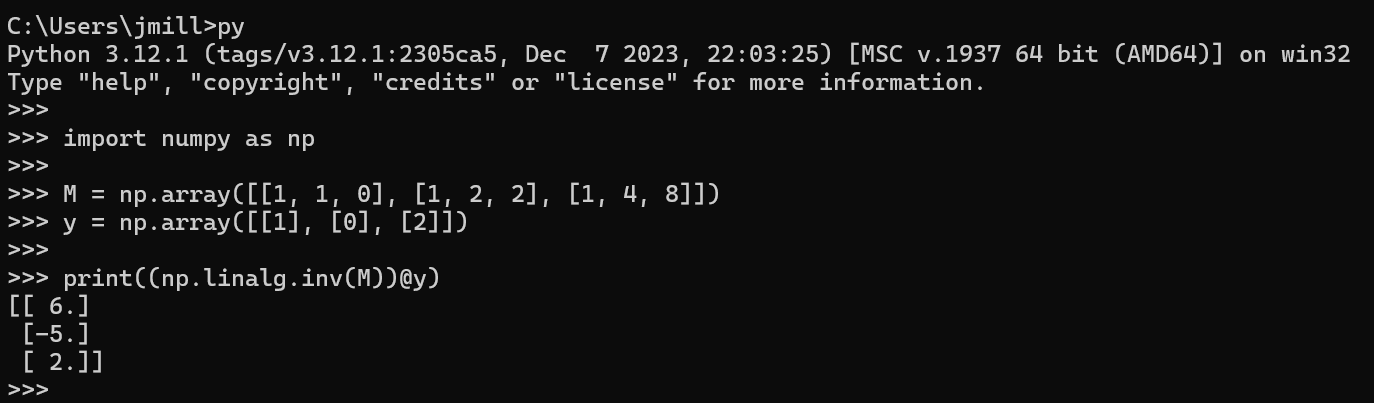
\includegraphics[scale=0.6]{188-HW1_Q1.png}\retTwo\par}

   So, $a_n = 6 - (5 + 2n)2^n$.\retTwo
\end{myIndent}

\blab{(2)} Let $(a_n)_{n\geq 0}$ and $(b_n)_{n \geq 0}$ be sequences. Assume that $(b_n)_{n \geq 0}$ satisfies a linear recurrence relation of order $e$. Then let $c_1, \ldots, c_d$ be scalars with $c_d \neq 0$ and assume that $(a_n)_{n \geq 0}$ satisfies:

{\centering $a_n = c_1a_{n-1} + \ldots + c_da_{n-d} + b_n$ for all $n \geq d$\retTwo\par}

Prove that $(a_n)_{n \geq 0}$ satisfies a linear recurrence relation of order $d + e$.

\begin{myIndent}\exOne
   To start, let's show some smaller facts:\retTwo

   \blab{Observation 1:} Suppose $a_n = c_1a_{n-1} + \ldots + c_da_{n-d} + p_m(n)r^n + F(n)$ where $F$ is some arbitrary function, $p_m$ is a polynomial of degree $m$ and $r$ is a nonzero constant. Then $a_n$ satisfies a recurrence relation of degree $e = d + m + 1$ where $F^\prime(n)$ is an arbitrary function $F(n)$ determined by $m$, $r$, and $F(n)$, and:
   
   {\centering $a_n = c^\prime_1 a_{n-1} + \ldots + c^\prime_e a_{n-e} + F^\prime(n)$ for all $n \geq e$.\newpage\par}
   
   \begin{myIndent}\exPP
         Proof by induction:\retTwo

         \blab{Lemma}: If $p_m(n)$ is a polynomial of degree $m > 0$, then $p_m(n) - p_m(n-1)$ is a\\ polynomial of degree $m - 1$.
         
         \begin{myIndent}\color{VioletRed}
            This is because for all $N > 0$ and coefficients $b$, we have that:\\ $bn^N - b(n - 1)^N = bn^N - bn^N + q(n)$ where $q$ is a polynomial\\ of degree $N - 1$. Meanwhile, the case where $N = 0$ is trivial.\retTwo
         \end{myIndent}

         \blab{Base Case:} If $m = 0$, meaning $p_m(n) = b$ where $b$ is a constant, then by taking the difference of $a_n$ and $r a_{n-1}$ for all $n \geq d + 1$, we get that:

         {\centering 
         \begin{tabular}{l}
            $a_n = (c_1 + r)a_{n-1} + (c_2 - rc_1)a_{n-2} + \ldots + (c_d - rc_{d-1})a_{n-d} - rc_da_{n-d-1}$\\ [4pt] $\phantom{Aaaaaaaaaaaaaaaaaaaaaaaaaaaaaaaaaaa} + F(n) - rF(n-1)$.
         \end{tabular} \retTwo\par}

         Setting $c_1^\prime = c_1 + 1, c_2^\prime = c_2 - rc_1,\phantom{.} \ldots,\phantom{.} c_d^\prime = c_d - rc_{d-1}, c_{d+1}^\prime = -rc_d$, and $F^\prime(n) = F(n) - rF(n - 1)$, we thus get that:

         {\centering$a_n = c_1^\prime a_{n-1} + \ldots + c_{d+1}^\prime a_{n-d-1} + F^\prime(n)$ for all $n \geq d + 1$.\par}
         
         \begin{myTindent}\begin{myDindent}\color{VioletRed}
            Also $c_{d+1}^\prime \neq 0$ because neither $r$ nor $c_d$ equal $0$.\retTwo
         \end{myDindent}\end{myTindent}

         
         \blab{Induction on $m$:} If $m > 0$, then by taking the difference of $a_n$ and $ra_{n-1}$ for all $n \geq d + 1$, since $r^n(p(n)) - rr^n(p(n-1)) = r^n(p(n) - p(n-1))$, we get by our lemma above that:\\ [-12pt]

         {\center
         \begin{tabular}{l}
            $a_n = (c_1 + r)a_{n-1} + (c_2 - rc_1)a_{n-2} + \ldots + (c_d - rc_{d-1})a_{n-d}$ \\ $\phantom{a_n = (c_1 + r)a_{n-1} + (c_2 - rc_1)a_{n-2}} - rc_da_{n-d-1} + q(n)r^n + F^\prime(n)$
         \end{tabular}\\ [6pt]\par}

         where $q$ is a polynomial of degree $m - 1$ and $F^\prime(n) = F(n) - rF(n-1)$.
         
         \begin{myDindent}\begin{myIndent}\color{VioletRed}
            And same as before, $-r c_d \neq 0$ because $r \neq 0$ and $c_d \neq 0$.\retTwo
         \end{myIndent}\end{myDindent}

         But now we can conclude by induction that $a_n$ satisfies a (possibly inhomogeneous) recurrence relation of order $e = (d + 1) + ((m - 1) + 1) = d + m + 1$ such that $F^\pprime(n)$ is some function determined by $m$, $r$ and $F(n)$, and:
         
         {\centering$a_n = c_1^\pprime a_{n-1} + \ldots + c_{e}^\pprime a_{n-e} + F^\pprime(n)$ for all $n \geq e$.\\ [26pt]\par}
   \end{myIndent}

   One important observation from above is that if $F(n) = 0$, then $F^\prime(n) = 0$. In some other situations, $F^\prime(n)$ also behaves nicely.\retTwo

   \blab{Observation 2:} Let $p_1(n), \ldots, p_k(n)$ be polynomials of degree $m_1, \ldots, m_k$ respectively. Also let $r_1, \ldots r_k$ be distinct nonzero constants. If:
   
   {\centering $a_n = c_1a_{n-1} + \ldots + c_da_{n-d} + p_1(n)r_1^n + F(n)$\\ \par}

   where $F(n) = \sum\limits_{i=2}^k p_i(n)r_i^n$, then part 1 will make  $F^\prime(n) = \sum\limits_{i = 2}^k q_i(n)r_i^n$ where\\ $q_2(n), \ldots, q_k(n)$ are also polynomials of degree $m_2, \ldots, m_k$ respectively.\\ [-6pt]

   \begin{myIndent}\exPP
      To see why, note that:
      
      {\centering $F(n) - r_1F(n -1) = \sum\limits_{i =2}^k p_i(n)r_i^n - \sum\limits_{i = 2}^k p_i(n - 1)r_1r_i^{n-1}$ \\
      $\phantom{F(n) - r_1F(n -1) = \sum\limits_{i =2}^k p_i(n)r_i^n} = \sum\limits_{i = 2}^k (p_i(n) - \frac{r_1}{r_i}p_i(n - 1))r_i^n$ \newpage\par}

      Because $r_i \neq r_1$, we know $\frac{r_1}{r_i} \neq 1$, meaning that the degree $m$ term of\\ $p_i(n) - \frac{r_1}{r_i}p_i(n - 1)$ doesn't cancel. So $q_i(n) \coloneq p_i(n) - \frac{r_1}{r_i}p_i(n - 1)$\\ is still a degree $m$ polynomial. If the process in part 1 takes more steps, then\\ we can just repeat this reasoning.\\ [6pt]
   \end{myIndent}

   Combining observations 1 and 2 together, we can inductively show that if
   
   {\centering $a_n = c_1a_{n-1} + \ldots + c_da_{n-d} + \sum\limits_{i = 1}^k p_i(n)r_i^n$\par}

   where $r_1, \ldots, r_k$ are distinct nonzero constants and $p_1(n), \ldots, p_k(n)$\\ [-6pt] are polynomials of degree $m_1, \ldots, m_k$ respectively, then letting $e = \sum\limits_{i=1}^k(m_i + 1)$,\\ [-6pt] there exists constants $c_1^\prime, \ldots c_{d + e}^\prime$ such that:

   {\centering $a_n = c_1^\prime a_{n-1} + \ldots + c_{e+d}^\prime a_{n-d-e}$ \retTwo\par}

   But now note that if $(b_n)_{n \geq 0}$ satisfies a linear recurrence relation of order $e$, we\\ [-2pt] can write $b_n = \sum\limits_{i = 1}^k p_i(n)r_i^n$ for some polynomials $p_1(n),\ldots p_k(n)$ with degrees\\ [-2pt] $m_1, \ldots, m_k$, as well as some distinct nonzero constants $r_1, \ldots, r_k$.
   
   \begin{myTindent}\exPP
      We know that each $r_i$ is nonzero because the constant term in the characteristic polynomial for $(b_n)$'s recurrence relation must be nonzero.\retTwo
   \end{myTindent}

   Also, as we showed in class, $\sum\limits_{i = 1}^k(m_i + 1) = e =$ the order of the recurrence relation\\ [-6pt] of $(b_n)_{n \geq 0}$.\retTwo

   So, we've shown that $a_n = c_1a_{n-1} + \ldots + c_da_{n-d} + b_n$ can be rewritten as a\\ homogenous linear recurrence relation of order $(d + e)$.\retTwo
\end{myIndent}

\blab{(3)} Let $(f_n)_{n \geq 0}$ be the Fibonacci numbers, and define $a_n = \sum\limits_{i = 0}^n f_i$.
\begin{itemize}
   \item[(a)] Find a linear recurrence relation of order $3$ that $(a_n)_{n \geq 0}$ satisfies.
   
   \begin{myIndent}\exOne
      Note that $(a_n)_{n \geq 0}$ satisfies the relation $a_n = a_{n - 1} + f_n$ for all $a_n$. Also, we showed in the first lecture that:

      {\centering $f_n = \frac{1}{\sqrt{5}}\left(\frac{1 + \sqrt{5}}{2}\right)^n - \frac{1}{\sqrt{5}}\left(\frac{1 - \sqrt{5}}{2}\right)^n $ \retTwo\par}

      So we know that: $a_n = a_{n-1} + \frac{1}{\sqrt{5}}\left(\frac{1 + \sqrt{5}}{2}\right)^n - \frac{1}{\sqrt{5}}\left(\frac{1 - \sqrt{5}}{2}\right)^n$\hspace{-0.4em}.

      Firstly, taking the difference of $a_n$ and $\frac{1 + \sqrt{5}}{2}a_{n-1}$, after a lot of simplifying we have that:
      
      \begin{myIndent}\exPP
         \begin{tabular}{l}
            $a_n = (1 + \frac{1 + \sqrt{5}}{2})a_{n-1} - \frac{1 + \sqrt{5}}{2}a_{n-2} + \left(-\frac{1}{\sqrt{5}} + \frac{1 + \sqrt{5}}{2\sqrt{5}}\cdot\frac{2}{1 - \sqrt{5}}\right)\left(\frac{1 - \sqrt{5}}{2}\right)^{n}$\\ [8pt]
            $\phantom{a_n} = \frac{3 + \sqrt{5}}{2}a_{n-1} - \frac{1 + \sqrt{5}}{2}a_{n-2} + \left(\frac{1 - \sqrt{5}}{2}\right)^{n-1}$
         \end{tabular}\newpage
      \end{myIndent}

      Secondly, we take the difference of $a_n$ and $\frac{1 - \sqrt{5}}{2}a_{n-1}$, and after a lot more\\ simplifying get:

      \begin{myIndent}\exPP
         \begin{tabular}{l}
            $a_n = \left(\frac{3 + \sqrt{5}}{2} + \frac{1-\sqrt{5}}{2}\right)a_{n-1} - \left(\frac{1 + \sqrt{5}}{2} + \frac{1-\sqrt{5}}{2}\cdot \frac{3+\sqrt{5}}{2}\right)a_{n-2} + \left(\frac{1-\sqrt{5}}{2}\cdot\frac{1 + \sqrt{5}}{2}\right)a_{n-3}$ \\ [8pt]
            $\phantom{a_n} = 2a_{n-1} + 0a_{n-2} - a_{n-3}$
         \end{tabular}\retTwo
      \end{myIndent}
   \end{myIndent}

   \item[(b)] Find a closed formula for $a_n$. 
   
   \begin{myIndent}\exOne
      \blab{Method 1:}\\
      The characteristic polynomial of $a_n = 2a_{n-1} - a_{n-3}$ is $t^3 - 2t^2 + 1$. Just by looking at it, I can already see that $(t - 1)$ is a factor of that polynomial. So after doing polynomial long division, we have that $(t - 1)(t^2 - t - 1) = t^3 - 2t^2 + 1$.\retTwo

      By quadratic formula, the remaining roots are $\frac{1 + \sqrt{5}}{2}$ and $\frac{1 - \sqrt{5}}{2}$ (a.k.a the same roots as with the Fibonacci recurrence relation).\retTwo

      Finally, we get a system of linear equations:
      
      {\centering$
      \begin{bmatrix}
         1 & 1 & 1 \\ 1 & \frac{1 + \sqrt{5}}{2} & \frac{1 - \sqrt{5}}{2} \\  1 & \left(\frac{1 + \sqrt{5}}{2}\right)^2 & \left(\frac{1 - \sqrt{5}}{2}\right)^2
      \end{bmatrix}
      \begin{bmatrix}
         \beta_1 \\ \beta_2 \\ \beta_3
      \end{bmatrix} = 
      \begin{bmatrix}
         0 \\ 1 \\ 2
      \end{bmatrix}$\retTwo\par}

      To solve this, I finally started learning sympy:

      {\centering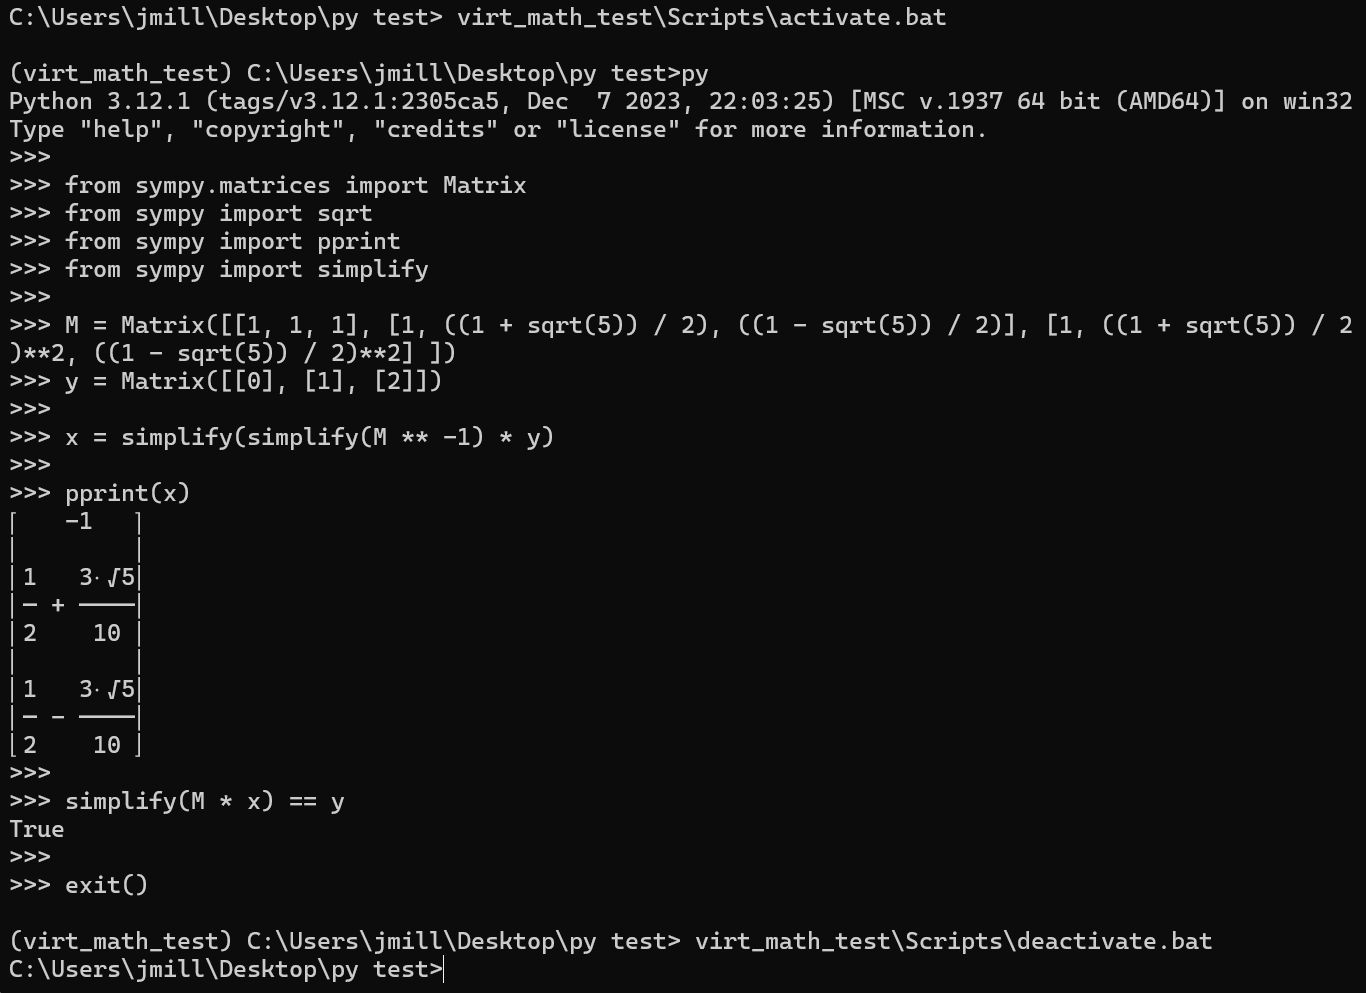
\includegraphics[scale=0.58]{188-HW1_Q3.png}\newpage\par}

      So, assuming I've not made a silly error somewhere, we should have that:

      {\centering $a_n = -1 + \left(\frac{5 + 3\sqrt{5}}{10}\right)\left(\frac{1 + \sqrt{5}}{2}\right)^n + \left(\frac{5 - 3\sqrt{5}}{10}\right)\left(\frac{1 - \sqrt{5}}{2}\right)^n$ \retTwo\par}

      \blab{Method 2: (The hinted route)}\\
      Note that $\frac{1 - r^{n+1}}{1-r} = \sum\limits_{i=0}^n r^i$. Using this fact, we can see that:

      {\centering\exPP
      \begin{tabular}{l}
         $a_n = \sum\limits_{i = 0}^n f_i = \frac{1}{\sqrt{5}}\sum\limits_{i = 0}^n\left(\frac{1 + \sqrt{5}}{2}\right)^i - \frac{1}{\sqrt{5}}\sum\limits_{i = 0}^n\left(\frac{1 - \sqrt{5}}{2}\right)^i$ \\ [10pt]
         $\phantom{a_n = \sum\limits_{i = 0}^n f_i} = \frac{1}{\sqrt{5}}\cdot \frac{1}{1 - \frac{1 + \sqrt{5}}{2}}\left(1 - (\frac{1 + \sqrt{5}}{2})^{n + 1}\right) - \frac{1}{\sqrt{5}}\cdot \frac{1}{1 - \frac{1 - \sqrt{5}}{2}}\left(1 - (\frac{1 - \sqrt{5}}{2})^{n + 1}\right)$
      \end{tabular}\retTwo\par}

      Now technically we are done since that is a closed formula for $a_n$. However, it looks ugly. So I'm going to learn more sympy so it can symplify this:

      {\centering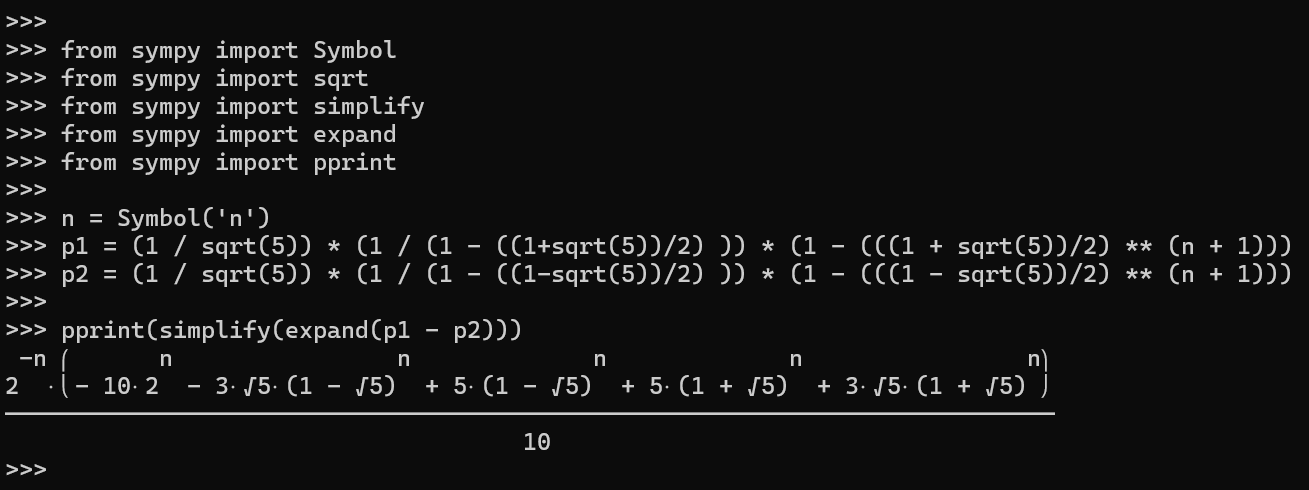
\includegraphics[scale=0.58]{188-HW1_Q3B.png}\retTwo\par}

      Hence we get the same answer as before:

      {\centering $a_n = -1 + \left(\frac{5 + 3\sqrt{5}}{10}\right)\left(\frac{1 + \sqrt{5}}{2}\right)^n + \left(\frac{5 - 3\sqrt{5}}{10}\right)\left(\frac{1 - \sqrt{5}}{2}\right)^n $ \retTwo\par}
   \end{myIndent}
\end{itemize}




\end{document}